\clearpage
\section{Website Downloads}
\label{sec:evaluation-website}

\begin{figure*}[!htb]
    \begin{minipage}[t]{0.8\linewidth}
	\begin{center}
        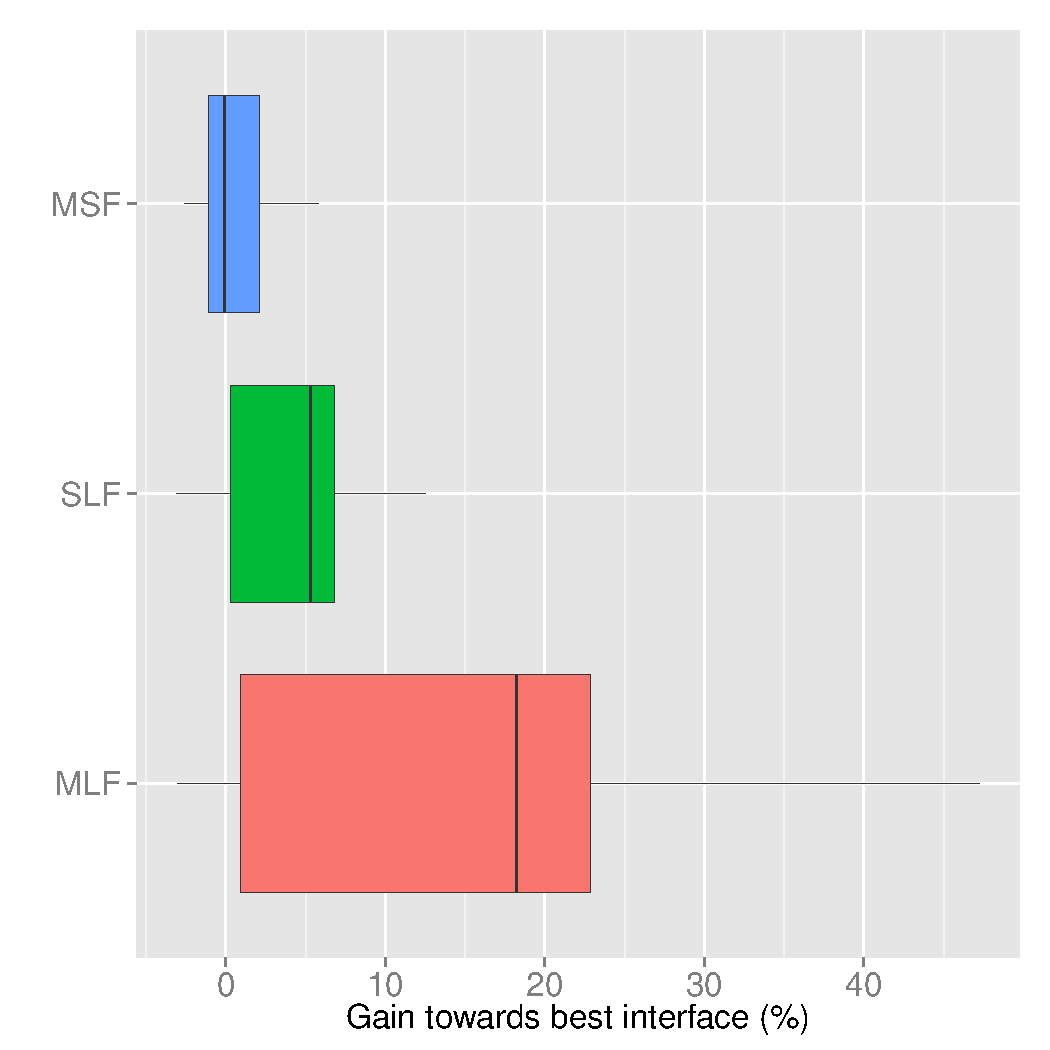
\includegraphics[width=\linewidth]{Figures/website-category-performance.pdf}
		\caption{\label{fig:website-performance-category}Performance gain (\perc) of each category towards best interface (\ethernet).}
    \end{center}
    \end{minipage}
\vspace*{-0.3cm}
\end{figure*}

Web pages differ in number and size of embedded files. 
\mhttp~is specifically designed for large files. 
Therefore, its general performance on websites is highly dependent on the portion of large embedded files. 
For a proper evaluation we select 24 web pages from \term{Alexa.com}~\cite{URL-ALEXA} and divide them into 3 categories. 
Each category is then evaluated separately, in order to study the effect of \mhttp~on different kinds of websites. 
As listed in~\tref{tab:website-category}, the categories are many small files (\term{MSF}), some large files (\term{SLF}) and 
many large files (\term{MLF}). 
The categorization is mainly based on the fraction of large files ($>$1MB) embedded in the page. 

%The performance of downloading web pages using \mhttp is significantly affected 
%by the size and number of embedded files. Therefore, the performance evaluation of
%\mhttp on random web pages cannot be seen as the general result. 
%Consequently, we divide web pages into three different categories according to the size 
%of the embedded objects and evaluate \mhttp over each category separately. The three 
%categories are many small files (\term{MSF}), some large
%files (\term{SLF}), and many large files (\term{MLF}). The categorization is mainly based on
%the fraction of large files ($>$1MB) embedded in the page. The categorization
%scheme and the number of samples are listed in~\tref{tab:website-category}.

A web page has to meet certain requirements in order to be used for our experiments.  
First, the content of a web page should not change too
frequently since our measurement is performed repeatedly in different time
periods. Second, the majority of embedded objects in the web page should not be
dynamically generated on every access request. Third, the majority of web
objects on the web server must be accessible through HTTP,~\ie no HTTPS-only
servers, without authentication. All 24 selected web pages fulfill these criteria. 
Note, that for this experiment all selected web pages are index pages. 
Index pages tend to have smaller embedded objects that can be quickly delivered to the user. 

%For our experiments, these pages are manually verified and selected to meet
%certain requirements. First, the content of a web page should not change too
%frequently since our measurement is performed repeatedly in different time
%periods. Second, the majority of embedded objects in the web page should not be
%dynamically generated on every access request. Third, the majority of web
%objects on the web server must be accessible through HTTP,~\ie no HTTPS-only
%servers, without authentication. As a result, we select 24 web pages in
%total.

\begin{figure*}[!htb]
    \begin{minipage}[t]{0.8\linewidth}
    \begin{center}
        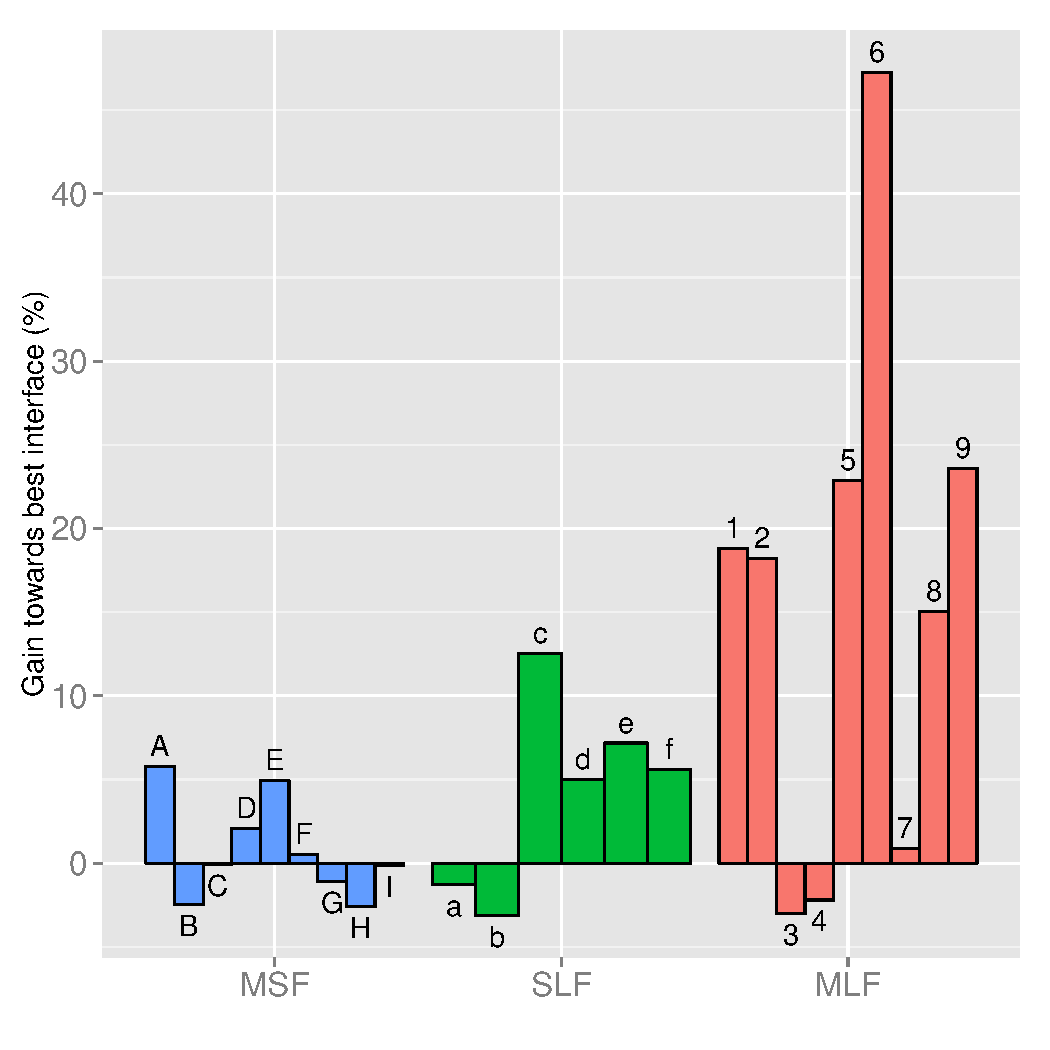
\includegraphics[width=\linewidth]{Figures/website-individual-performance.pdf}
		\caption{\label{fig:website-performance-site}Performance gain (\perc) of each website towards best interface (\ethernet).}
    \end{center}
    \end{minipage}
  \vspace*{-0.3cm}
\end{figure*}

Our previous experiments were conducted in controlled testbeds in Germany and in the US. 
For the web performance experiment we use a laptop equipped with an \ethernet~interface and a \wifi~interface, both connected to the Internet via two different access networks. 
The laptop is located in a German university campus. 
Similar like with our controlled German testbed, we throttle the \ethernet~and \wifi~interface to 15Mbps and 10Mbps respectively, in order to simulate a more common environment. 
We use \mhttp~with an initial chunk size of $32$KB and the \algslice~scheduler, due to the reasons explained in~\xref{sec:evaluation-schedulers-mixed} and~\xref{sec:evaluation-initial-chunk}.
$\alpha_{i,j}$ is set to $20$, as explained in~\xref{sec:evaluation-alpha}.

%Unlike our previous experiments that were performed in controlled testbeds in Germany and in the US, the
%web workload experiment is conducted in a German university campus using a
%laptop equipped with an \ethernet~interface and a \wifi~interface connected to
%the Internet via two different access networks. We use \mhttp~with
%an initial chunk size of $32$KB and the \algslice~scheduler, due to reasons explained in~\xref{sec:evaluation-schedulers-mixed} and~\xref{sec:evaluation-initial-chunk}.
%$\alpha_{i,j}$ is set to $20$, as explained in~\xref{sec:evaluation-alpha}.

\fref{fig:website-performance-category} and~\fref{fig:website-performance-site} illustrate the performance gain and
loss of \mhttp~in web page downloads compared to HTTP over the best performing
interface (\ethernet~in our experiment).
As expected, we observe essentially no gain for the \term{MSF} category. 
This category has no large files embedded, which is why this result is not surprising. 
The \term{SLF} and \term{MLF} category web sites on the other hand gain around $5$\perc and $18$\perc respectively. 

%\fref{fig:website-performance} (a) and (b) illustrate the performance gain and
%loss of \mhttp~in web page downloads compared to HTTP over the best performing
%interface (\ethernet~in our experiment). From the results we observe that 
%there is essentially no gain for websites in the \term{MSF} category, a gain of around $5$\perc for 
%those in the \term{SLF} category, and around $18$\perc for websites in the \term{MLF} category. The lack of 
%a performance gain for the \term{MSF} category is not surprising since web pages that belong 
%to this category do not embed any large files. 

\fref{fig:website-performance-site} depicts the performance gain achieved for each individual 
website in each category. The web page, alias \emph{A} in the \term{MSF}
category in~\fref{fig:website-performance-site} shows good performance even without
any large files. On closer investigation, we find that the web
page embeds many files that are smaller than $1$MB, but much larger than the
initial chunk size. 

\begin{table}[!htb]
\begin{center}
\tabcolsep3mm
\begin{tabular*}{0.98\linewidth}{lrrr}
\toprule
                                             & \scriptsize{\term{MSF}}      & \scriptsize{\term{SLF}}                & \scriptsize{\term{MLF}}  \\
\midrule
\scriptsize{\perc of large files ($>$ 1 MB)} & \scriptsize{0\perc}   & \scriptsize{$<$ 1\perc}         & \scriptsize{$>$ 1\perc} \\
\scriptsize{Median(\perc of large files)}    & \scriptsize{0\perc}   & \scriptsize{$0.59$\perc}  & \scriptsize{$2.5$\perc} \\
\scriptsize{No. of samples (pages)}          & \scriptsize{9} & \scriptsize{6}           & \scriptsize{9}        \\
%\multicolumn{4}{l}{}\\
\bottomrule
\end{tabular*}
\end{center}
\caption{Web page categorization scheme}
\label{tab:website-category}
\vspace{-3mm}
\end{table}

For websites in the \term{SLF} and \term{MLF} categories, we observe a significant performance 
gain using \mhttp. 
This is especially true for the \term{SLF} category where the fraction of large files is less than $1$\perc. 
Here, one of the web pages (\emph{c} in~\fref{fig:website-performance-site}) shows more than $10$\perc gain using \mhttp. 
Considering the small difference between the percentage of large files in \term{SLF} (median $0.59$\perc) and in \term{MLF} (median $2.5$\perc), the difference in the median gain between the two categories is significantly high. 
In particular, web page \emph{6} embeds around $2.5$\perc of large files and has a median file size of around $170$KB and exhibits almost $50$\perc of the performance gain by using \mhttp.
This shows that \mhttp~does not harm the browsing of web pages with no large files, but it has the potential to greatly decrease the download times of web sites with large embedded ones and already a small fraction of large embedded objects is sufficient, to witness a gain. 

%This shows again the well-known fact that while there may be many small files, 
%large files are responsible for the bulk of the total value traffic in the Internet.
%Hence, multipath approaches such as \mhttp~can bring significant decreases 
%in download times to users.
